\documentclass{report}
  \usepackage[utf8x]{inputenc}
  \usepackage{mathtools}
  \usepackage{listings}
  \usepackage{graphicx}
  \usepackage[titletoc]{appendix}
  \graphicspath{ {./diagrams/} }
  \usepackage{url}
  \title{Temporal Innovation on the Blockchain}
  \author{ChronoLogic}
  \date{\today\\v0.9}
  \begin{document}
  \maketitle
  \begin{abstract}
    Current generation blockchains lack the crucial time-based functionality like transaction scheduling. The proposed paper discusses potential implementable solutions and challenges for enabling such a functionality.
  \end{abstract}
  \newpage
  \tableofcontents
  \newpage
  \chapter{Introduction}
  Scheduling is a feature that is native to the modern financial world.
  We schedule our routine bank transfers and bill payments; whenever we know ahead of time when a payment should go through, we set it up to pay automatically instead of waiting for the exact time and date. Financial transactions are increasingly moving to the self-sovereign and trustless world of cryptocurrencies. As more volume is moved on networks like Ethereum\footnote{\url{https://www.ethereum.org/}} daily, there is more expectation of the foundational tooling that fiat world provides. Users expect scheduling as a feature from the Ethereum ecosystem because they have learned to rely on it in their everyday lives. In fact, scheduling calls on Ethereum is more powerful than scheduling movements of money in the fiat world -- users can now schedule smart contracts execution. They have access to much more complex logic. We also identify the tooling gap that exists for developers working on the Ethereum stack, used to cron jobs on Unix. Contrary to intuition, scheduling calls on a decentralized peer-to-peer blockchain is not a trivial problem to solve.

  There are many reasons why a person would want to schedule smart contract calls. The most facile of use cases involves the simple scheduling of value transfers -- the movement of ether or an ERC20 token from one address to another. With the future indoctrination of concepts such as DAOs\footnote{\url{https://en.wikipedia.org/wiki/Decentralized_autonomous_organization}}, the world will start to see smart contracts employed in the use of organizational governance and other high stakes uses. Users may want to schedule a vote to a DAO for instance that will determine the zoning of their neighborhood that they live in. Additionally, developers may invent new use cases in which scheduling is used under the hood, without the user even realizing the complexity behind the application that they are interacting with. Blockchains are the new software platform. People who set up and maintain software environments use cron\footnote{\url{https://en.wikipedia.org/wiki/Cron}} to schedule jobs (commands or shell scripts) to run periodically at fixed times, dates, or intervals. There needs to be a cron for the world of Ethereum.
  \section{Centralized Scheduling}
  On Ethereum there does not exist any native way to have a smart contract be called at a specified time in the future, or to make this call recurring. The obvious need for this feature has led developers to create their own solutions. In the (now deprecated) Parity UI\footnote{\url{https://github.com/paritytech/parity-ui}} there was a built-in scheduling feature that would locally hold the transaction in memory before sending it at the desired time. Although the solution worked fine, there were some major drawbacks including 1) the necessity of the user running their own local node and using the specific Parity client software, and 2) the single point of failure experienced in the instance that the local node disconnected from the peer-to-peer network. These multiple issues can actually be composed into one: centralization.
  \section{Decentralized Scheduling}
  The advantages of a decentralized protocol over a centralized one is that it does not have a single point of failure. The scheduling aspect of the Ethereum Alarm Clock\footnote{The Ethereum Alarm Clock was created by Piper Merriam, now Lead of the Python team at Ethereum, on August 26, 2015. Throughout its development history it was deployed to the Ethereum network and maintained almost solely by a single developer. The adoption of the protocol did not take off and after the 2016 DDoS attacks on the Ethereum network the smart contracts started to fall out of date as Piper began pursuing new projects} is done entirely through smart contracts running on Ethereum on the backend and allows for permission-less implementations of user-friendly front-ends \footnote{Among two of the already implemented front-ends on the current iteration of the Ethereum Alarm Clock are the ChronoLogic Chronos Dapp \url{https://app.chronologic.network} and a native integration with the popular MyCrypto wallet \url{https://mycrypto.com}}. The execution aspect of the protocol is handled by a network of off-chain clients known as TimeNodes. TimeNodes are incentivized to operate by the user-set bounty payment, which can be thought of as a small reward provided by the user for the TimeNode to expense its own computation costs for monitoring the state of Ethereum. From a user perspective, the existence of TimeNodes never has to be known and they can pay the small premium of the bounty without any understanding of the execution flow of the Ethereum Alarm Clock protocol entirely.
  \chapter{Ethereum Alarm Clock}
  In November 2017, nearly one year after the DDoS attacks that metaphorically threw a ratchet in the Ethereum Alarm Clock’s gears, developers from the ChronoLogic team began to work on and reboot the Ethereum Alarm Clock protocol. After about nine months of work including updating the core smart contracts, rewriting the test suite in JavaScript for the Truffle framework, building developer libraries and constructing a new TimeNode client in TypeScript, and performing numerous internal audits and an external audit with a notable member of the community, the ChronoLogic team deployed the 1.0.0 stable release of the Ethereum Alarm Clock smart contracts on August 24, 2018. The following information will discuss the architecture, analyze the cryptoeconomic incentives, and enumerate on some of the limitations found in the stable release.
  \section{Architecture}
  The Ethereum Alarm Clock architecture is best described in two symbiotic and differential parts-- the smart contracts which are deployed to the Ethereum main chain and operate trustlessly and the TimeNode network, which are off-chain execution agents in charge of handling the logic of executions.
  \begin{figure}[h]
  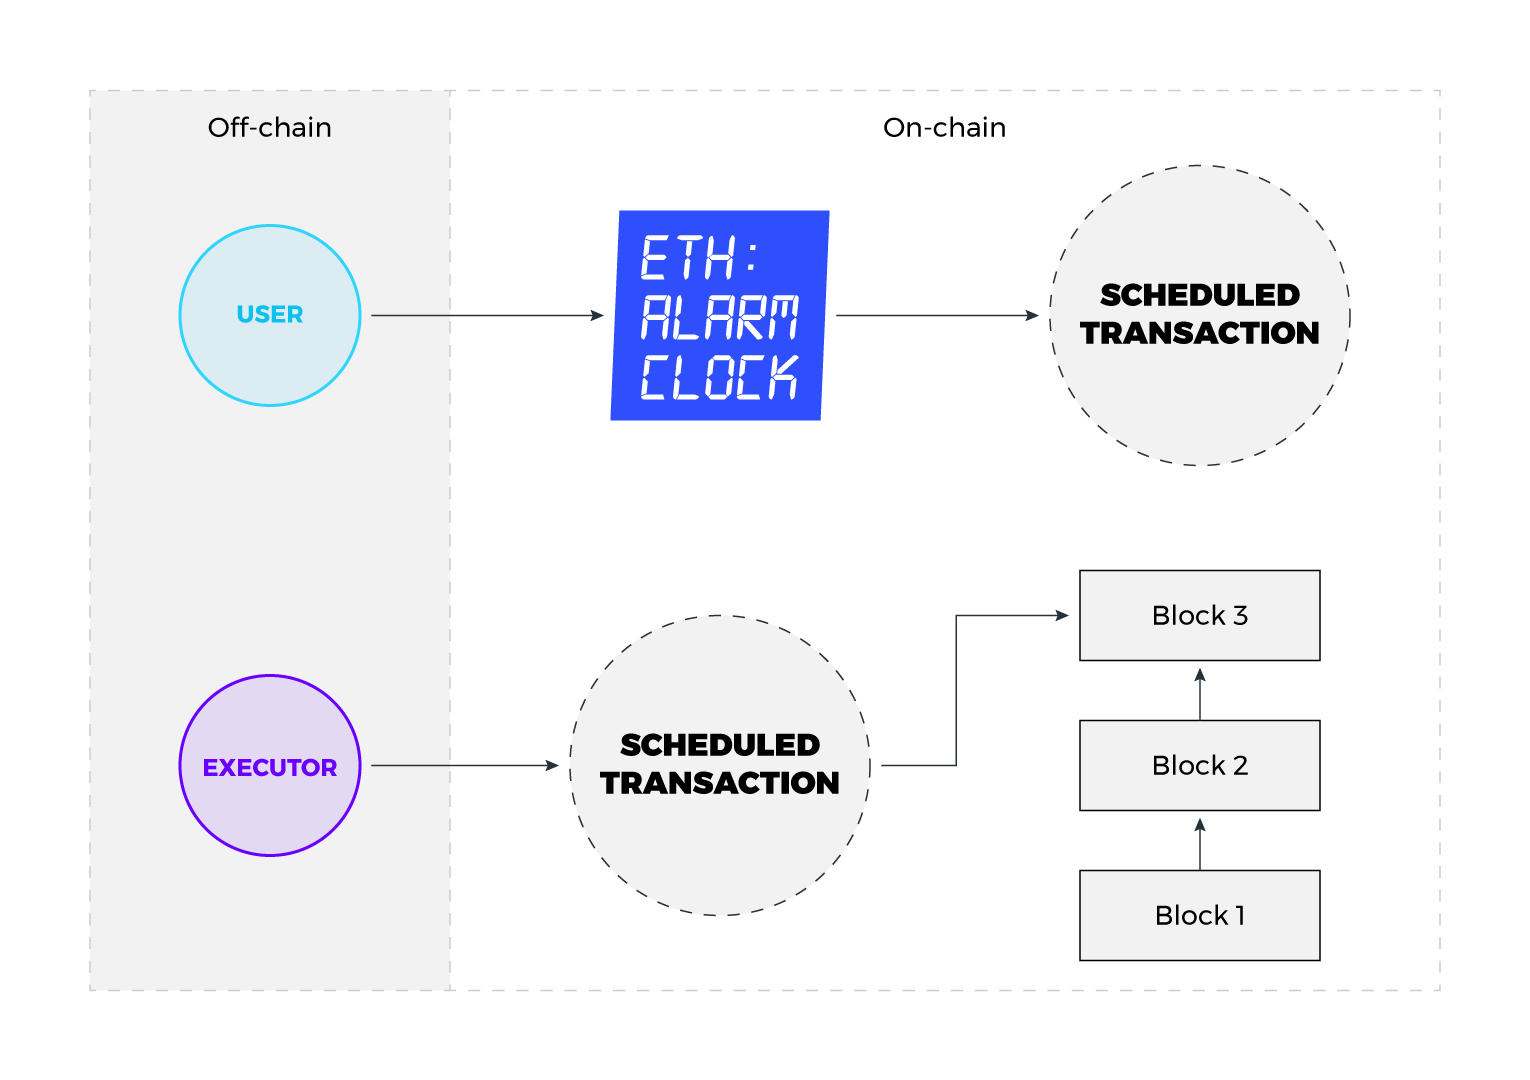
\includegraphics[width=\textwidth]{diagram6}
  \caption{Ethereum Alarm Clock architecture overview}
  \end{figure}
  \subsection{Smart Contracts}
  The smart contracts of the Ethereum Alarm Clock can be thought of as consisting mainly of three parts: \textbf{RequestFactory}, \textbf{Schedulers} (further divided into the TimestampScheduler and BlockScheduler), and \textbf{TransactionRequestCore}. Within these three main sections of the architecture are numerous libraries that contain various pieces of the core logic and functionality. There are nine library contracts, two top-level scheduler contracts, on contract for \textbf{RequestFactory} and one for \textbf{TransactionRequestCore}, adding in Zeppelin’s SafeMath and Ownable brings the total to 15 smart contracts which compose the entire Ethereum Alarm Clock architecture.

  \begin{figure}[h]
    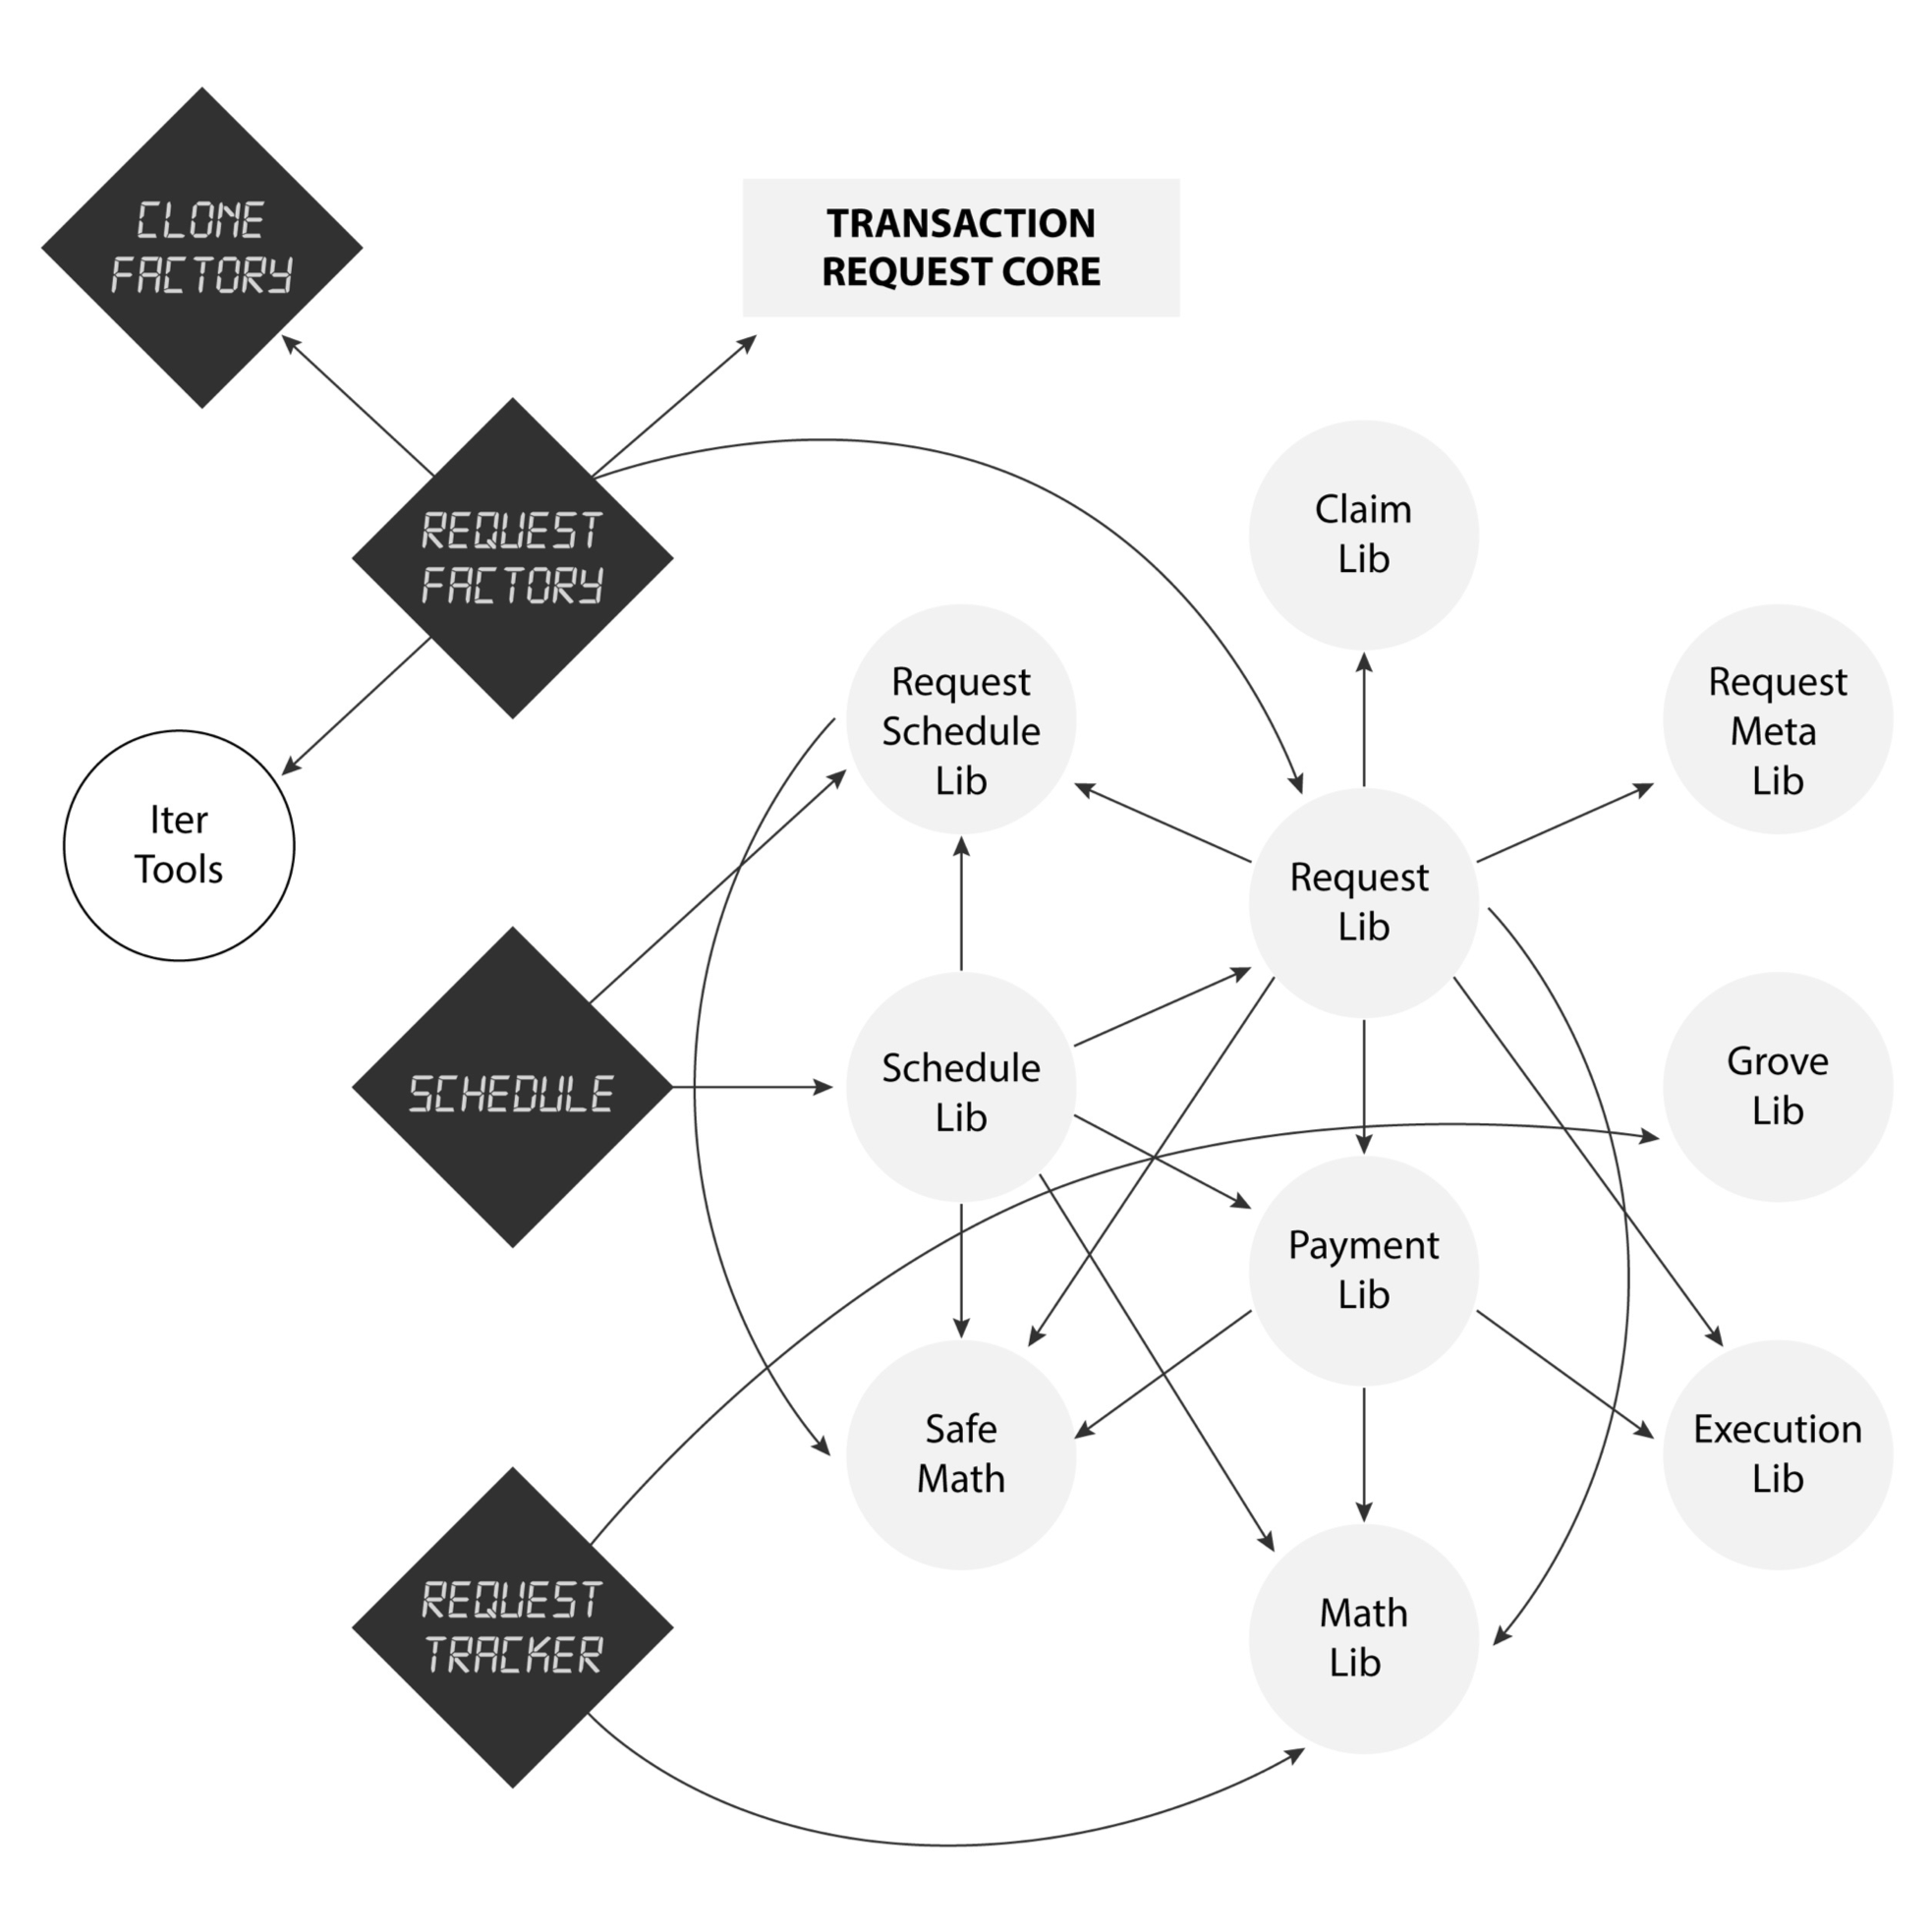
\includegraphics[width=\textwidth]{contracts}
    \caption{Ethereum Alarm Clock smart contracts overview}
  \end{figure}

  The logic for the scheduled transactions exist on the \textbf{TransactionRequestCore} contract which acts as the central library for the numerous instances of the \texttt{delegatecall}\footnote{\url{https://github.com/ethereum/EIPs/issues/23}} clone contracts that get deployed via the \textbf{RequestFactory}. Below is shown the code example of the primary actions of the \textbf{TransactionRequestCore}, which allows TimeNodes to execute, cancel or claim a scheduled transaction.
  \begin{verbatim}

   function execute() public returns (bool);
   function cancel() public returns (bool);
   function claim() public payable returns (bool);

  \end{verbatim}

  The \textbf{Schedulers} (\textit{BlockScheduler.sol} and \textit{TimestampScheduler.sol}) are the top level APIs which will get exposed to the user facing applications. These contracts provide a simpler interface taking only the necessary parameters for a scheduled transaction and setting the rest of the options to sane defaults. The \textbf{Scheduler} contracts are also the objects which hold the data concerning the taking of fees. The purpose of separating the logic for taking fees into the Scheduler contracts is to allow third party developers and new integrations to customize their fee structure (and fee destination) in their own preferred way. Allowing the option for third party integration to customize their fee structures creates an incentive for them to make the integration into their own product. Each scheduler contracts works off the same \textbf{RequestFactory} backend so it benefits from the same network of TimeNodes.

  The \textbf{RequestFactory} contract is the core of the Ethereum Alarm Clock protocol and deploys the new \texttt{delegatecall} clone contracts. It is possible to call the Request Factory directly but most of the time the Request Factory will be called by an “internal transaction” by one of the Scheduler contracts. The \textbf{RequestFactory} has two functions which perform different kinds of validation of the parameters which are passed in. The lower level \texttt{`createRequest()`} will attempt the raw creation of a \textbf{TransactionRequest} without any validation. By not performing validation the function call saves gas but may lead to the possibility that the parameters contained an error and will not be executed properly. For most use cases some validation of the input parameters is desired and the \texttt{`createValidatedRequest()`} will be used instead. The \textbf{RequestFactory} will also be the factory that TimeNodes watch in order to keep up to date with scheduled transactions since it emits the \texttt{`RequestCreated`} event which alerts TimeNodes of user scheduled transactions.

  \subsection{TimeNode}
  TimeNodes are the off-chain execution agents which represent individual nodes of the decentralized peer-to-peer execution network behind the Ethereum Alarm Clock.

  \begin{figure}[h]
    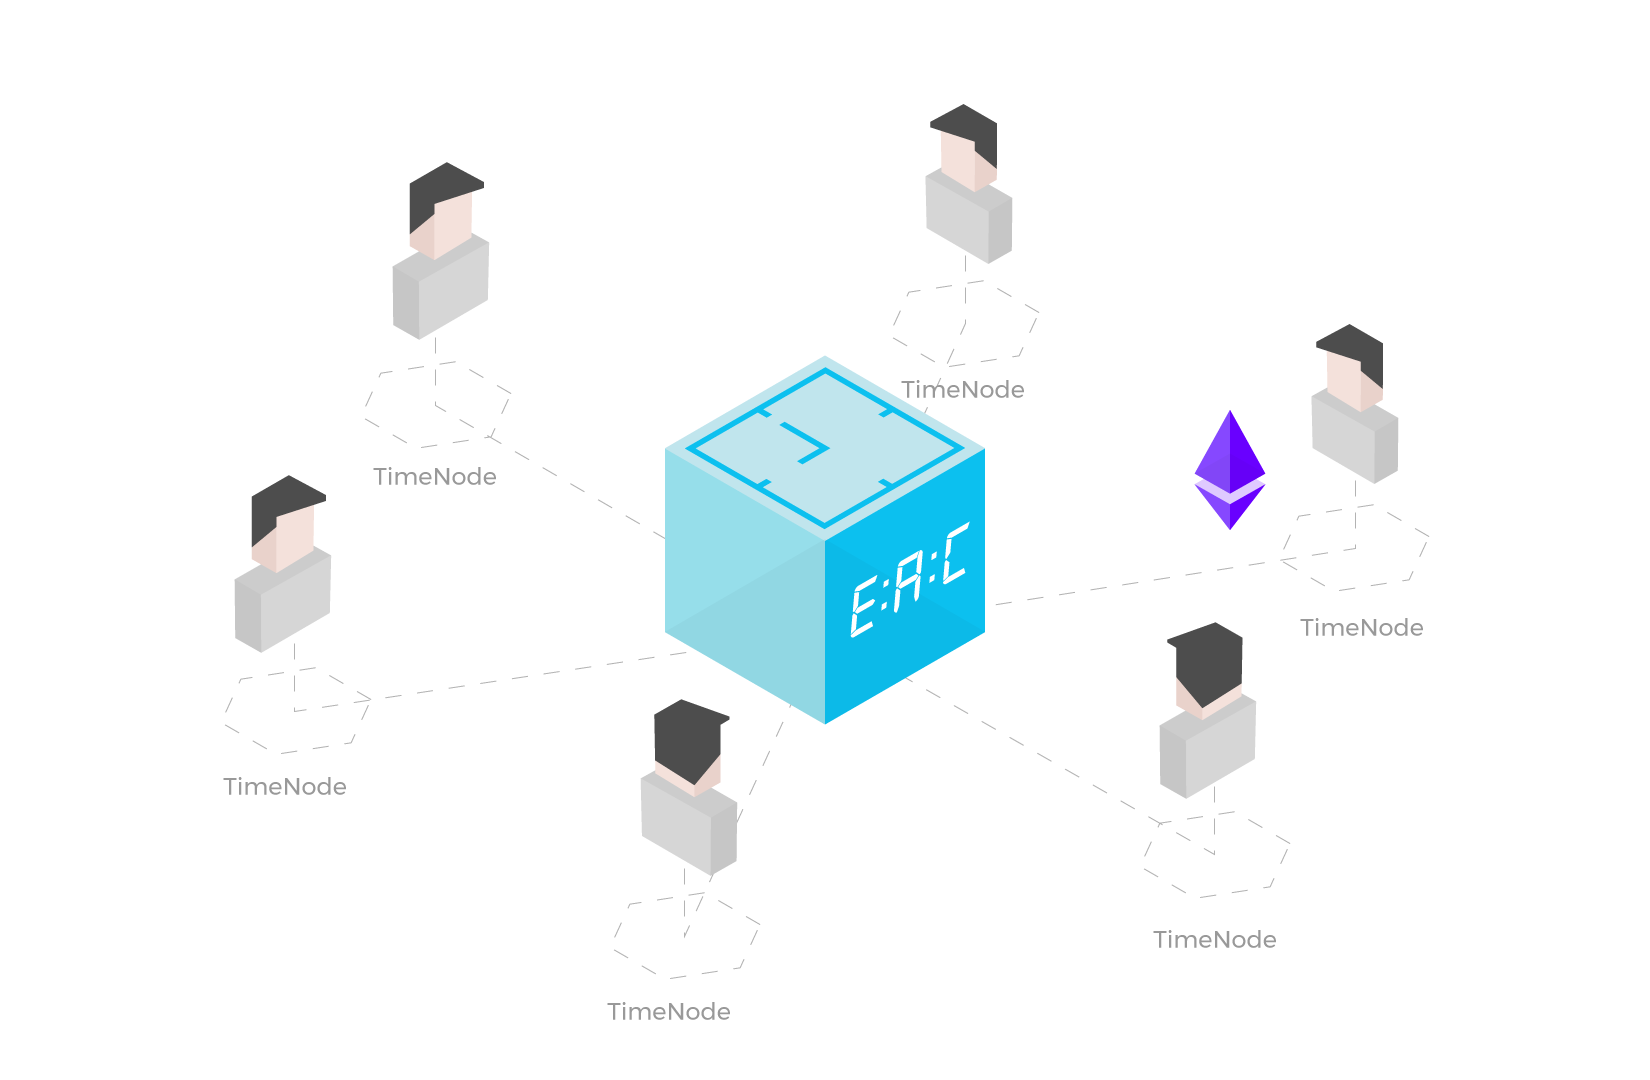
\includegraphics[width=\textwidth]{diagram1}
    \caption{Ethereum Alarm Clock TimeNodes network}
  \end{figure}

  The first and primary TimeNode action is the execute function while the second action is claim - which well go into detail in the next section. Execute is called anytime a TimeNode tries to execute a transaction that has been scheduled to be executed.

  By executing a transaction, a TimeNode receives a reward (bounty). This helps incentivize TimeNodes to execute incoming scheduled transactions.

  The execute action is run by triggering a function within the smart contract that holds the scheduled transaction. This trigger requires the TimeNode to spend a small amount of gas to trigger this action.

  A problem arises when multiple TimeNodes send the execute trigger at the same time, i.e. within the same block. Only one of them will trigger the execution, while the other TimeNode’s transaction will get reverted and cost a small amount of gas.

  Should a TimeNode notice that it often collides with other TimeNodes during the execution time of scheduled transactions, it can choose to claim transactions.

  \section{Claiming Mechanism}
  Claiming is an advanced opt-in feature of the Ethereum Alarm Clock protocol which helps TimeNodes lower the risk of transaction collisions.

  When users schedule a transaction, this scheduled transaction appears on the blockchain and TimeNodes keep track of them. Once it is scheduled, a TimeNode can attempt to claim the scheduled transaction by depositing a small amount of ETH.

  Claiming transactions removes the risk of colliding with other TimeNodes during the execution time, but brings forward another set of problems:
  \begin{enumerate}
    \item Transaction collisions - The same transaction collisions that used to happen on the execute function will now be a problem with the claim function. There is a chance of multiple TimeNodes trying to claim the same transaction within the same block, which will again result in a transaction collision and only one of those will be able to claim it.
    \item Deposit loss - When a TimeNode claims a transaction it deposits a small amount of ETH as a guarantee that it will be online to execute it when the time is right. Should a TimeNode (due to unforeseen circumstances) go offline at the exact time at which the scheduled transaction was due to be executed, it will lose its deposit.
  \end{enumerate}
  \section{Remote Providers}
  The effect of sending the claim or execute actions for a scheduled transaction can bring more risks, depending on whether a TimeNode is connected to a local or a remote node.

  Connecting the TimeNode to a remote provider can introduce delays due to network conditions and can facilitate failed claims/executions. Running a local RPC provider node would be the recommended way of running the TimeNode to eliminate the risk of slow responses for the RPC requests made by the TimeNode.
  \section{Mitigation Efforts}
  Efforts have been made to mitigate the risks mentioned above by introducing the hasPending check to the timenode-core library. hasPending allows the TimeNodes to check the transaction pool (txpool) of the providers it is connected for any incoming execute or claim actions on a certain scheduled transactions.

  This allows the TimeNodes to avoid transaction collisions if they use a node that has a txpool such as Parity or Geth. Keep in mind that RPC providers without a txpool (e.g. Infura over HTTP) will not work with this feature.

  \section{Recommendation}
  In order to avoid the mentioned risks of running a TimeNode, we recommend the following setup:
  \begin{itemize}
    \item Connect the TimeNode to a local Parity/Geth node
    \item Turn on claiming transactions
    \item Reliable internet connection - minimum offline time
  \end{itemize}

  These risks are currently unquantifiable and it is still not clear how the network will behave in real world conditions.

  \section{Cryptoeconomics}
  The Ethereum Alarm Clock protocol incorporates cryptoeconomic incentives to reward the decentralized network of TimeNodes to continue operation. The incentive consists of the extra amount of ether sent to the TimeNode following an execution. The amount of the bounty is variable and depends on when the transaction was claimed as well as how much extra gas was paid for the execution of the transaction. As a general rule, TimeNodes will not execute transactions which will return a net loss to their ETH balance. The formula for the bounty calculation is provided below.
  \begin{align*}
    &B_{total} = P \times B_{set} - (G_{actual} - G_{set})
  \end{align*}

  where $P$ is payment modifier

  Given that scheduled transactions are expected to be executed at the exact time and the network of n competing nodes exists, we expect to face the ”swarming” problem which can be described as: uncoordinated attempts of execution by n nodes at the same time. This problem may result in unnecessary costs for TimeNode making the operations potentially not profitable as only 1-of-n is going to earn the TimeBounty for the execution, other TimeNodes trying to execute at the same block will pay the failing transaction cost. By introducing payment modifier P TimeNode operators are able to pick theirs profitability point, this effectively allows to mitigate the ”swarming” problem as we expect TimeNodes to try to claim on different blocks/moment of time. However, under perfect competition, the profitability metric of the TimeNode trends toward perfect zero leading TimeNodes to often send claim transaction within the same block.

  For detailed economic for TimeNodes refer to appendix \ref{appendix}.
  \section{Limitations}
  \subsection{Gas price}
  The Ethereum network uses the concept of gas as a unit of measuring the computational work performed over the network. Every transaction broadcasted to the network sets the gas limit and the gas price. Gas limit describes the maximum amount of gas allowed to be consumed by the transaction, gas price describes the amount of ether (ETH) you are willing to pay for each unit of gas.

  While setting the gas limit is in most cases very straightforward and automatic, setting the correct gas price is not a trivial task. Gas price determines the time between broadcasting and block inclusion, depends on current network capacity. We observed many spikes in the gas price due to popular ICOs\footnote{\url{https://en.wikipedia.org/wiki/Initial_coin_offering}}, CryptoKitties or last FCoin on-chain voting.
Given the nature of scheduled transactions, protocol needs to handle the execution using predicted gas price. The most important characteristics are:
  \begin{itemize}
    \item execution prioritization
    \item TimeNode withholding protection
  \end{itemize}

  There are three possible solution for this problem, lets analyze each of them separately:

  \begin{enumerate}
    \item
      Fixed gas price - Allows setting the gas price that has to be used by TimeNode for execution, declared gas price is reimbursed by the scheduler

      Pros:
      \begin{itemize}
        \item simple
        \item protects from TimeNode withholding
      \end{itemize}
      Cons:
      \begin{itemize}
        \item fails upon gas price spikes
        \item requires users to guess the price in the future
      \end{itemize}

    \item
      Range gas price - Allows setting minimum and maximum gas price by the scheduler, the maximum gas price is reimbursed, any gas price used by the TimeNode between min and max (spot price) will allow the split of the remaining budget between the scheduler and the TimeNode.

      \textit{For e.g, the scheduler sets the range from 20gwei to 100gwei and thus locks enough funds to cover 100gwei * gas limit. TimeNode is incentivized to pick a good price between 20 and 100, let’s say 50 as remaining 50 is split, making TimeNode earn extra 25.}

      Pros:
      \begin{itemize}
        \item protects from TimeNode withholding
        \item incentivize TimeNodes to pick correct price within bounds
      \end{itemize}
      Cons:
      \begin{itemize}
        \item given the front-running, the equilibrium is max
        \item requires a decently high max in order to cover the spikes
      \end{itemize}

    \item
      Minimum gas price - Allows setting the minimum gas price by the scheduler, the minimum gas price is reimbursed, higher gas prices covered by TimeNode (effectively reducing the reward for execution)

      Pros:
      \begin{itemize}
        \item protects from TimeNode withholding
        \item allows the TimeNode to decide where equilibrium is
      \end{itemize}
      Cons:
      \begin{itemize}
        \item covers spikes up the minimum reimbursement + reward
      \end{itemize}
  \end{enumerate}

  In order to pick the right solution we need understand the Ethereum Alarm Clock execution process. There are 3 different time windows used for:
  \begin{itemize}
    \item pre-execution claiming process: where TimeNodes are bidding on reservation for execution
    \item reserved execution: time period for TimeNode that claimed transaction
    \item execution: free for all execution, when TimeNode that claimed missed the execution or no claiming happened
  \end{itemize}
  Minimum gas price is the best option for both reserved execution and execution as it allows TimeNodes to control and pick the gas price that best fits their own profit model.

  \subsection{Account abstraction}
  For cases where the address of the sender has to be known upfront and given the Ethereum Alarm Clock architecture where each scheduled transaction is represented by separate smart contract and have unique Ethereum address there is a need to use a proxy wallet.
  Proxy wallet address will be seen as msg.sender in destination contract/account. An example procedure off scheduling transaction using proxy wallet could be described as follows:
  \begin{enumerate}
    \item create schedule request such as the destination is set to proxy wallet
    \item send scheduling request using proxy wallet so it becomes the owner of the request
    \item whitelist the scheduled request in the proxy wallet so it can be relayed
  \end{enumerate}

  The need for such a workaround will not be necessary when native account abstraction \footnote{https://github.com/ethereum/EIPs/issues/859} will be available on Ethereum network.

  \subsection{Gas cost}
  Using smart contract storage for keeping data with conditions and parameters for scheduled transaction comes with a cost. Currently each scheduled transaction costs approximately 500 000 gas. Even though the total cost in USD is below \$1\footnote{Given current 8.2Gwei gas price} the “premium” for scheduling is over 20x comparing to regular ETH transfers.

  \section{DAY token}

  Running the web\footnote{\url{https://app.chronologic.network}} and desktop\footnote{\url{https://github.com/chronologic/eth-alarm-clock-dapp/releases}} version of TimeNode software requires users to prove the ownership of 333 DAY\footnote{\url{https://etherscan.io/token/0xE814aeE960a85208C3dB542C53E7D4a6C8D5f60F}} tokens. The required amount can be hold on any Ethereum account controlled by the TimeNode operator.

  \chapter{Chronos - Next generation scheduling protocol}
  \section{Conditional scheduling}

  Time-based scheduling is a very powerful idea, but it’s not capable of handling \texttt{if-this-then-that} type of scheduling. The idea to explore this type of scheduling was sparked by discussions with teams and projects in the Ethereum space about potential use-cases for the Ethereum Alarm Clock. Some of them were based on a state change, rather than a specific time period.

  Let’s take a closer look at the example on how we could implement decentralized stop-loss functionality using the Ethereum Alarm Clock. One of the possible solutions for the problem that could be implemented can be defined as follows:

  \begin{itemize}
    \item Create a smart contact called StopLoss with execute function that is going to check a decentralized exchange for your current position and will place the sell order if certain conditions are met
    \item Use the Ethereum Alarm Clock protocol to create a scheduled transaction with recurring execution for \texttt{execute} for e.g every 5min
  \end{itemize}

  While this solution works, it would generate an enormously high cost for users, given 500000gas the daily cost is approximately
  \[
    ~500 000 gas \times 12 \times 24 \approx \$130\footnote{Given 1ETH = 221USD and GasPrice=4.1GWei}
  \]

  making this it not feasible.

  In general, the problem with this approach is that every trigger costs gas regardless of whether it succeeds or not. A much more efficient solution for this problem would be to have a scheduler that allows one to store conditions directly in the contract and allows the execution only when these conditions are met.

  Looking through that lens we came to the conclusion that time-based scheduling is just a special case of conditional scheduling. The conditions are: \texttt{if time then} or \texttt{if block then}. TimeNodes (the off-chain executors) are checking time and block conditions before the execution (by reading them from the smart contract) which means that they attempt the sending of transactions only when those conditions are met. Instead of defining time or block we delegate this check to external contracts that for e.g has method \texttt{inExecutionWindow(uint windowStart, uint windowSize) returns (bool)} which check whether \texttt{block.number} if within the given window.

  \section{DAY token staking}

  Ethereum Alarm Clock protocol is using claiming process in order to improve cryptoeconomics by reducing the collision among the TimeNodes. Chronos protocol will take different approach to solve this problem, we are designing claiming mechanism based on DAY token staking.

  Staking model assumes that DAY tokens act as an collateral for claiming actions and align the incentives for execution. Any commitment by the TimeNode would have to be backed by amount of DAY tokens, lack of execution will result in token slashing. Whether complete stake or partial slashing, it is still to be seen.

  The Priority Queue based approach to stake can be described as follows:

  \begin{itemize}
    \item Client running TimeNode software must first register their intent to be a claiming TimeNode on the blockchain by sending a transaction containing some amount of tokens to a contract. Inside of this transaction, the TimeNode specifies its preferences for what kinds of transactions it wants to execute. These preferences include how big of a bounty is attached to the \textbf{ScheduledTransaction} and when the execution window starts.
    \item Each time a TimeNode enters the \texttt{Claiming Queue} the entry with the highest amount staked is moved to the top of the queue while all other entries are sorted downward.
    \item When a user wants to schedule a transaction, they send a transaction to the Chronos \textbf{Scheduler} contract containing the data of the transaction they would like executed at a later time (or when later conditionals return true).
    \item The next TimeNode on the \texttt{Claiming Queue} which fits the preferences of that TimeNode will be popped off the queue and “assigned” to that transaction.
    \item Upon execution time, that TimeNode which was assigned has the exclusive rights to send the \texttt{execute} transaction and the other TimeNodes will not even try.
  \end{itemize}

  \chapter{Second Layer Execution Markets}
  \section{Delegated execution}
  Delegated execution in a pattern that is used by both Ethereum Alarm Clock, Chronos and others\footnote{Gnosis Safe, uPort relayers...}. On the high level, it enables safe transaction delegation to 3rd party agents in exchange for the reward.

  \begin{figure}[h]
    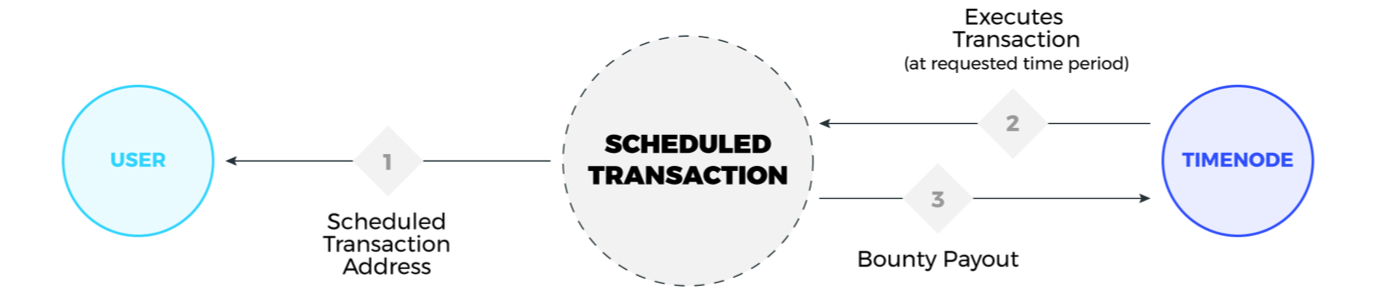
\includegraphics[width=\textwidth]{delegated_execution}
    \caption{Delegated execution example}
  \end{figure}

  \section{Execution market}

  Currently in the Ethereum ecosystem there are multiple projects working on their own execution markets for their purpose. The drawback of this approach is that the economic incentive to participate in such market depends on the amount of delegation available. Protocols and DApps\footnote{\url{https://en.wikipedia.org/wiki/Decentralized_application}} will scatter the market into smaller ones, potentially not profitable to join.

  \begin{figure}[h]
    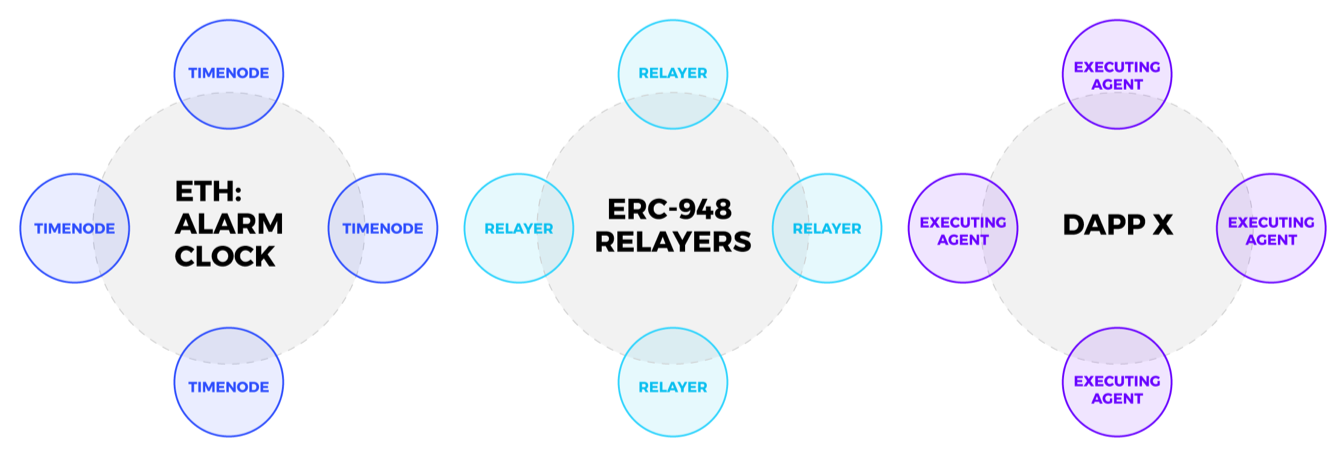
\includegraphics[width=\textwidth]{silos}
    \caption{Siloed relayers markets}
  \end{figure}

  The issues with the siloed markets are:
  \begin{itemize}
    \item Amount of nodes depends on amount of bounties
    \item Reliability of the network depends on amount of nodes
    \item Networks run by the protocol and DApps creators are subject to low censorship resistance
  \end{itemize}

  The solution for this would be to conceptualize the common market that is able to handle multiple protocols and DApps.

  \begin{figure}[h]
    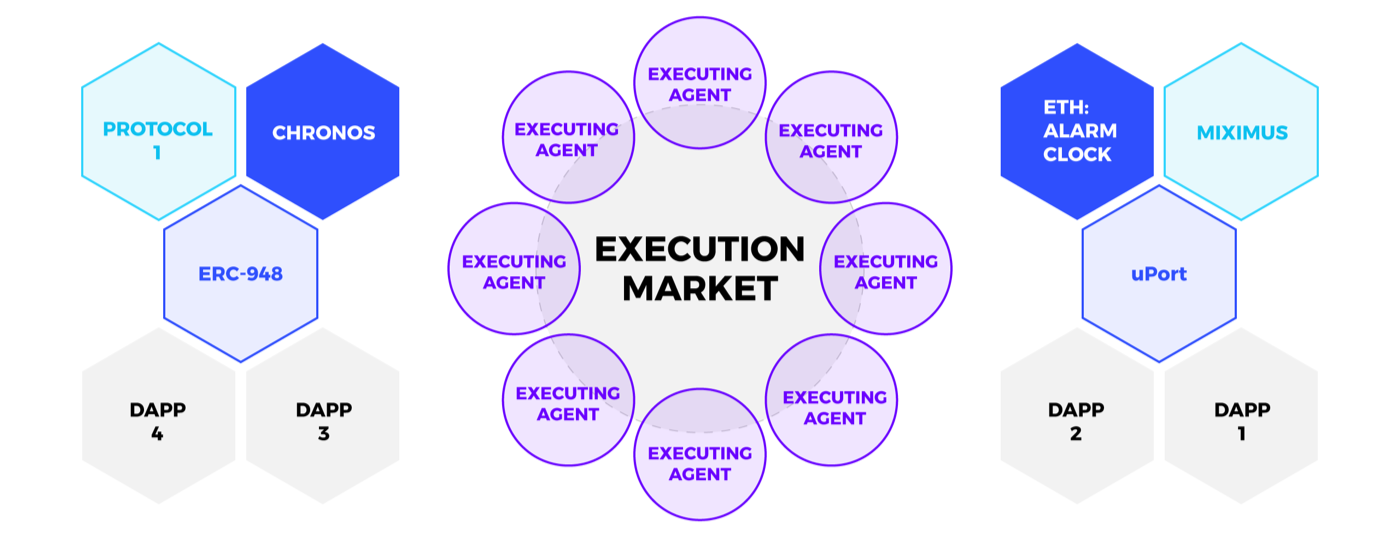
\includegraphics[width=\textwidth]{comon}
    \caption{Common relayers markets}
  \end{figure}

  In order to design such a market there are few pre-conditions:

  \begin{itemize}
    \item Agree on interfaces for off-chain and on-chain representations (EIP-1077\footnote{\url{https://eips.ethereum.org/EIPS/eip-1077}} and ERC-1228\footnote{\url{https://github.com/ethereum/EIPs/issues/1228}})
    \item Agree on bounties representation (ERC-1197\footnote{\url{https://github.com/ethereum/EIPs/issues/1197}})
  \end{itemize}

  \section{TimeNode - beyond the scheduling}

  \begin{appendices}
    \chapter{The on-chain claiming mechanism economics}\label{appendix}
    \section{Claiming mechanism}
  Claiming mechanism can be described as follows:
  For any transaction $Tx$ that has been deployed to the network and is expected to be executed by 1 of $n$ nodes in the network. The process of execution is divided into two steps:
  \textbf{claiming} and \textbf{execution}. Claiming is a process of reserving the transaction for further execution.
  \begin{figure}
    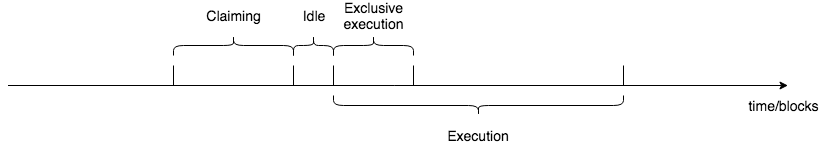
\includegraphics[width=\linewidth]{claiming/timeranges.png}
    \caption{Scheduled transaction life cycle}
    \label{fig:boat1}
  \end{figure}

  \subsection{Claiming}
  \begin{itemize}
  \item can happen before execution
  \item every node has the same chance to successfully claim $Tx$
  \item claiming requires a $Deposit$ to be locked by claimant
  \item $Deposit$ is lost by claimant when execution won't happen within \textit{exclusive execution window}
  \item every node can fail on claiming when $Tx$ was already claimed
  \item claiming requires sending transaction that has cost described as $C_{c}$ when success and $C_{f}$ when failure
  \item payment modifier $P_{mod}(t)=\begin{cases}
  0 & \quad \text{at beginning of claiming window}\\
  1 & \quad \text{at end of claiming window}
  \end{cases}$
  \item claiming is optional
  \end{itemize}

  \subsection{Execution}
  \begin{itemize}
  \item successful execution has reward described as $TimeBounty$
  \item execution cost is reimbursed by the scheduler when successful
  \item execution cost has cost described as $C_{e}$ when not successful
  \item $Deposit$ locked by the claimant can be acquired by a node when the claimant failed to execute
  \end{itemize}

  \subsection{Expected payout definition}
  Let's define the expected payout for node as
  \[
  P=P_{s}+P_{f}+P_{nf}
  \]
  where
  \\

  $P_{s}$ is expected payout after successful claiming and execution
  \\

  $P_{f}$ is expected payout after successful claiming and missed execution
  \\

  $P_{nf}$ is expected payout after other node losing the deposit
  \\

  \subsubsection{Network with $n=1$ nodes}
  For network of nodes with $n=1$ we can define expected payouts as:
  \[
  P_{s}(P_{mod})=P_{mod} \times TimeBounty-C_{C}
  \]
  \[
  P_{f}=-C_{C}-Deposit
  \]
  \[
  P_{nf}=TimeBounty-C_{C}
  \]
  \subsubsection{Network with $n>1$ nodes}
  For that case the expected reward will be $\frac{TimeBounty}{n}$ assuming that probability of successful claiming is equal for all nodes. Also in case of failing transaction node will pay the $C_{Tx}$
  \[
  P_{s}(P_{mod})=\frac{P_{mod} \times TimeBounty-C_{C}}{n} - (n-1) \times C_{Tx}
  \]
  \[
  P_{f}=-C_{C}-Deposit
  \]
  \[
  P_{nf}=\frac{TimeBounty+Deposit}{n} - (n-1) \times C_{Tx}
  \]

  In order to improve the cost of failing transactions let's introduce a mechanism $X$ that prevents sending the transaction that will fail, the accuracy of mechanism $X$ is defined as $A_{X} \in [0;1]$

  \[
  P_{s}(A_{X}, P_{mod})=\frac{P_{mod} \times TimeBounty-C_{C}}{n} - (1-A_{X}) \times (n-1) \times C_{Tx}
  \]
  \[
  P_{f}=-C_{C}-Deposit
  \]
  \[
  P_{nf}(A_{X})=\frac{TimeBounty+Deposit}{n} - (1-A_{X}) \times (n-1) \times C_{Tx}
  \]

  The last part is to introduce $P_{ld} \in [0;1]$ as probability of TimeNode loosing the $Deposit$


  \[
  \label{eq}
  P(A_{X}, P_{ld}, P_{mod})=P_{s}(A_{X}, P_{mod}) \times (1-P_{ld}) + (P_{f}(A_{X})+P_{nf}(A_{X})) \times P_{ld}
  \]
  \section{Simulation}
  We are going to simulate few cases using equation formulated in section \ref{eq}. $A_{X}, P_{ld}, P_{mod}$ are the variables that depends on reliability and running costs by TimeNode owners. All calculated results are going to be represented as \textit{gas}

  Let's now define the profitability threshold. We will assume monthly running cost for the TimeNode is 7USD (this is based on current rates on Heroku cloud). Translating 7USD to \textit{gas} we get:

  \begin{align*}
  ETH/USD=700USD\\
  Gas Price = 10Gwei\\
  7USD \equiv 1000000gas
  \end{align*}

  This shows us that running costs are covered after acquiring 1000000\textit{gas}. Now let's take a look at how this translates to the amount of executed transactions. In order to calculate $P(A_{X}, P_{ld}, P_{mod})$ we use the script listed below. Moreover we are using following values describing TimeNode operations and network conditions:
  \begin{align*}
  &n \approx 8\\
  &TimeBounty \approx 300000gas\\
  &Deposit \approx 600000gas\\
  &A_{X} \approx 0.95 (95\%)\\
  &P_{ld} \approx 0.1 (1\%)\\
  &C_{C} = 90000gas\\
  &C_{Tx} = 25000gas\\
  &target = 1000000gas~or~7USD
  \end{align*}
  Results using these parameters are:
  \begin{verbatim}
       p_mod       res  tx
    15  0.70  1428.250 700
    16  0.75  3178.094 314
    17  0.80  4450.974 224
    18  0.85  5951.569 168
    19  0.90  7394.698 135
    20  0.95  8980.225 111
    21  1.00 10402.272  96
  \end{verbatim}
  Results data frame contains 3 columns:
  \begin{itemize}
  \item \textbf{p\_mod} - payment modifier ($P_{mod}$)
  \item \textbf{res} - expected amount of gas earned by TimeNode per transaction
  \item \textbf{num\_of\_tx} - number of transactions to be executed in order to cover running costs
  \end{itemize}

  The results achieved by running this simulation should be treated informational rather than something taken for granted. The expected payout depends on all of the variables described above, for a simulation purpose we picked values using our intuition.

  The variable controlled by the TimeNode operator is $P_{mod}$ which is the major component. Low enough $P_{mod}$ allows TimeNode to claim transaction before others, still, in order to be profitable using low $P_{mod} $, the TimeNode running cost has to be low.

  The TimeNode market has many characteristics of the perfect competition market\footnote{\url{http://www.economicsonline.co.uk/Business_economics/Perfect_competition.html}}: there is perfect information, no barriers to entry, they deliver the same service, TimeNode are the price takers. Based on that, long-term we may get in the situation where marginal cost is equal average cost.
  \end{appendices}
  \end{document}
